\documentclass[a4paper, 11pt, final, garamond]{book}
\usepackage{cours-preambule}

\raggedbottom

\makeatletter
\renewcommand{\@chapapp}{Programme de kh\^olle -- semaine}
\makeatother

\begin{document}
\setcounter{chapter}{29}

\chapter{Du 12 au 16 juin}

\section{Cours et exercices}
\section*{Architecture de la matière ch.3 -- Solides cristallins}
\begin{enumerate}[label=\Roman*]
	\litem{Différents types de solides}~: solides cristallins, amorphes,
	semi-cristallins~; allotropie.
	\litem{Modèle du cristal parfait}~: description (réseau, motif, maille),
	mailles cubiques (CS, CC, CFC), dénombrement (population, coordinence),
	occupation du volume (compacité, masse volumique), limite du modèle.
	\litem{Cristal parfait de sphères dures}~: modèle, empilements compacts (ABA,
	ABC), condition de contact et application calculs de compacité (CS, CC,
	CFC), sites interstitiels (définition, habitabilité, sites O et T)~:
	position, nombre de sites par maille et habitabilité.
	\litem{Différents types de cristaux}~: métalliques (description, propriétés
	macro) et alliages, ioniques (description, propriétés macro) et exemples
	(\ce{CsCl}, \ce{NaCl}, \ce{ZnS}), covalents (description, propriétés,
	application diamant), moléculaires (description, propriétés macros) et bilan.
\end{enumerate}

\section{Cours uniquement}
\begin{center}
	\begin{framed}
		\Large \bfseries
		Exercices possibles à partir de mardi soir
	\end{framed}
\end{center}
\section*{Induction chapitre 1 -- Champs magnétiques}
\begin{enumerate}[label=\Roman*]
	\litem{Introduction}~: notion de champ, interaction entre aimants, vecteur
	champ magnétique.
	\litem{Sources et cartes de champ magnétique}~: aimant droit, lignes de
	champ~; champs magnétiques créés par des courants~: bobine plate, solénoïde.
	\litem{Intensité du champ magnétique}~: lire une intensité sur une carte,
	champs uniformes (bobines de \textsc{Helmoltz}), lien entre courant et champ
	magnétique~: règles de la main droite, proportionalité, symétries,
	invariances, exercice bilan.
	\litem{Le moment magnétique}~: boucle de courant, cas des aimants.
\end{enumerate}

\section*{Induction chapitre 2 -- Actions mécaniques du champ magnétique}
\begin{enumerate}[label=\Roman*]
	\litem{Observations expérimentales}~: aimant, rails de \textsc{Laplace}.
	\litem{Force de \textsc{Laplace}}~: densité linéique, expression intégrale et
	puissance, règle de la main droite.
	\litem{Couple de \textsc{Laplace}}~: spire rectangulaire dans champ constant,
	couple résultant et puissance associée.
\end{enumerate}

\section{Questions de cours possibles}

\begin{enumerate}[label=\sqenumi]
	\item[] \textbf{AM. chapitre 3}

		% \item Présenter le modèle du cristal parfait. Présenter les mailles cubiques
		%   classiques. Rappeler (et démontrer) les fondamentaux de géométrie d'un cube.
		%   Définir la population, la coordinence, la compacité et la masse volumique.
		%   Présenter le modèle des sphères dures, la condition de tangence et indiquer
		%   l'endroit de tangence pour les 3 mailles cubiques.

	\item Décrire la maille cubique faces centrées. Déterminer sa population, sa
	      coordinence, sa compacité. \textbf{Application}~: le fer $\gamma$ est une
	      variété allotropique du fer, cristallisant dans une structure CFC. Sa masse
	      volumique vaut $\rho = \SI{8.21e3}{kg.m^{-3}}$. Déterminer le paramètre de
	      la maille $a$ et de rayon $r$ des atomes de fer dans la structure. On donne
	      $M_{\ce{Fe}} = \SI{56}{g.mol^{-1}}$ et $\mathcal{N}_A =
		      \SI{6.02e23}{mol^{-1}}$.

	\item Présenter et justifier l'existence des sites interstitiels. Donner les
	      positions et la population des sites O et T de la structure CFC, et déterminer
	      leurs habitabilités.

	      \bigbreak

	\item[] Donner la population, la coordinence, la relation entre les rayons et
		le paramètre de maille, exprimer la compacité et la masse volumique et
		donner les propriétés macroscopiques d'un des cristaux suivants~:

	\item Le diamant~;
	\item Le chlorure de césium~;
	\item Le chlorure de sodium~;
	\item La blende.

	\item[] \textbf{Induction chapitre 1}

	\item Définir les lignes de champ et donner leur propriété pour le champ
	      $\vv{B}$. Dessiner les lignes de champ pour un aimant droit, une bobine
	      plate, un solénoïde et un aimant en U. Pour les champs issus d'un courant,
	      le lien entre l'orientation du courant et du champ $\vv{B}$ doit bien
	      évidemment être respecté.

	\item Indiquer comment lire une intensité sur une carte de champ, trois
	      manières de faire un champ uniforme, donner un ordre de grandeur de
	      l'intensité du champ pour 4 situations particulières (aimant, électroaimant,
	      IRM, champ terrestre), et refaire l'exercice~:
\end{enumerate}
\noindent
\begin{texem}{Exercice bilan}
	Les cartes de champ magnétique ci-dessous sont des vues en coupe du champ
	produit par des spires de courant circulaires. Dans les deux cas, indiquer 1/ la
	position des sources, 2/ le sens du courant circulant dans les spires, 3/ les
	zones de champ fort et faible, et 4/ le cas échéant s'il existe une zone de
	l'espace où le champ magnétique est uniforme.
	\begin{center}
		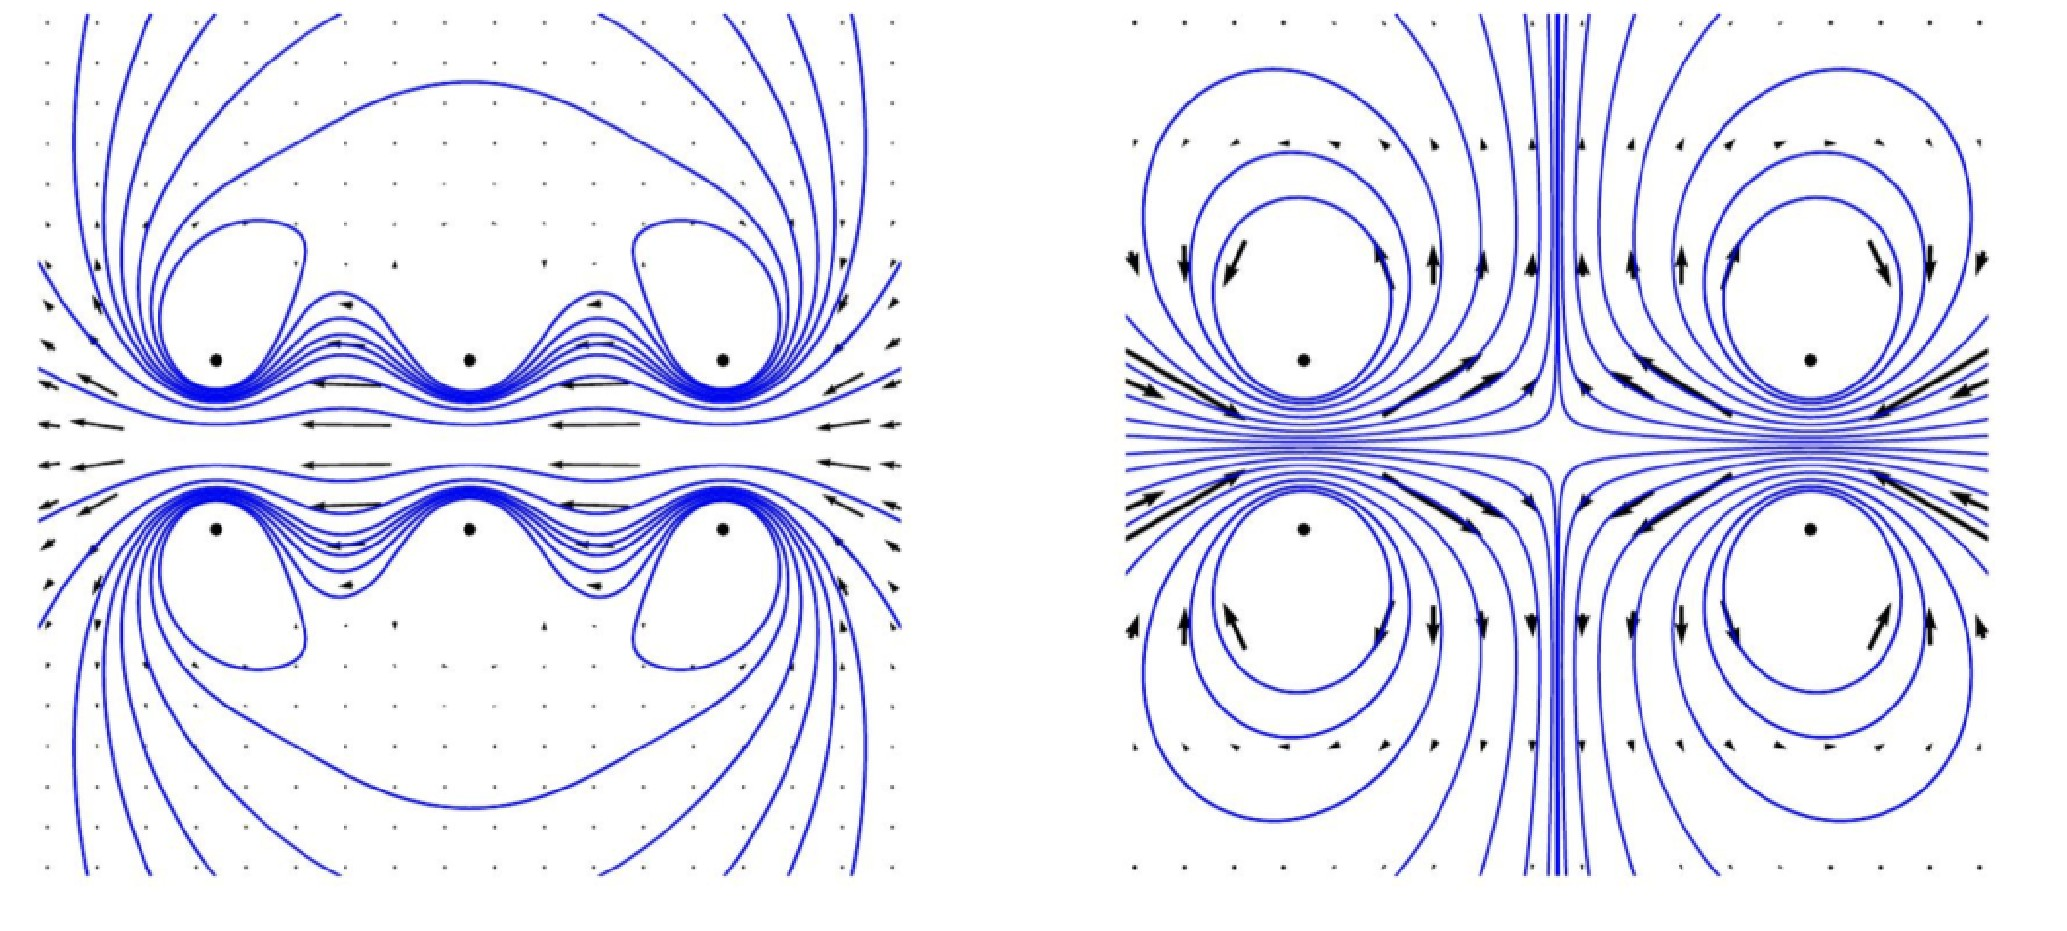
\includegraphics[scale=.8]{../figures/ch30/ldc_bilan}
	\end{center}
\end{texem}
\begin{enumerate}[resume, label=\sqenumi]
	\item[] \textbf{Induction chapitre 2}
	\item Démontrer les expressions linéique et intégrale de la force de
	      \textsc{Laplace} dans une barre conductrice soumise à un champ magnétique
	      uniforme et stationnaire. Exprimer alors la puissance de la force de
	      \textsc{Laplace}. À l'aide d'un schéma, expliquer l'expérience des rails de
	      \textsc{Laplace}.
	\item Établir le couple des actions de \textsc{Laplace} sur une spire
	      rectangulaire parcourue par un courant $I$ en rotation autour d'un axe de
	      symétrie orthogonal, et plongée dans un champ magnétique extérieur uniforme et
	      stationnaire. Au moins un calcul utilisera le bras de levier. En déduire la
	      puissance du couple.
\end{enumerate}

\vfill

\begin{center}
	\begin{framed}
		\Large
		Merci, et bonne fin d'année à touz~!
	\end{framed}
\end{center}

\vfill

\end{document}
